\documentclass[12pt,t]{beamer}
\usepackage{graphicx}
\usepackage{tikz}
\setbeameroption{hide notes}
\setbeamertemplate{note page}[plain]
\usepackage{listings}

% header.tex: boring LaTeX/Beamer details + macros

% get rid of junk
\usetheme{default}
\beamertemplatenavigationsymbolsempty
\hypersetup{pdfpagemode=UseNone} % don't show bookmarks on initial view


% font
\usepackage{fontspec}
\setsansfont
  [ ExternalLocation = fonts/ ,
    UprightFont = *-regular ,
    BoldFont = *-bold ,
    ItalicFont = *-italic ,
    BoldItalicFont = *-bolditalic ]{texgyreheros}
\setbeamerfont{note page}{family*=pplx,size=\footnotesize} % Palatino for notes
% "TeX Gyre Heros can be used as a replacement for Helvetica"
% I've placed them in fonts/; alternatively you can install them
% permanently on your system as follows:
%     Download http://www.gust.org.pl/projects/e-foundry/tex-gyre/heros/qhv2.004otf.zip
%     In Unix, unzip it into ~/.fonts
%     In Mac, unzip it, double-click the .otf files, and install using "FontBook"

% named colors
\definecolor{offwhite}{RGB}{255,250,240}
\definecolor{gray}{RGB}{155,155,155}

\ifx\notescolors\undefined % slides
  \definecolor{foreground}{RGB}{255,255,255}
  \definecolor{background}{RGB}{24,24,24}
  \definecolor{title}{RGB}{107,174,214}
  \definecolor{subtitle}{RGB}{120,120,120}
  \definecolor{hilit}{RGB}{102,255,204}
  \definecolor{vhilit}{RGB}{255,111,207}
  \definecolor{codehilit}{RGB}{255,111,207}
  \definecolor{lolit}{RGB}{155,155,155}
\else % notes
  \definecolor{background}{RGB}{255,255,255}
  \definecolor{foreground}{RGB}{24,24,24}
  \definecolor{title}{RGB}{27,94,134}
  \definecolor{subtitle}{RGB}{120,120,120}
  \definecolor{hilit}{RGB}{122,0,128}
  \definecolor{vhilit}{RGB}{255,0,128}
  \definecolor{codehilit}{RGB}{24,24,24}
  \definecolor{lolit}{RGB}{95,95,95}
\fi
\definecolor{nhilit}{RGB}{128,0,128}  % hilit color in notes
\definecolor{nvhilit}{RGB}{255,0,128} % vhilit for notes

\newcommand{\hilit}{\color{hilit}}
\newcommand{\vhilit}{\color{vhilit}}
\newcommand{\nhilit}{\color{nhilit}}
\newcommand{\nvhilit}{\color{nvhilit}}
\newcommand{\lolit}{\color{lolit}}

% use those colors
\setbeamercolor{titlelike}{fg=title}
\setbeamercolor{subtitle}{fg=subtitle}
\setbeamercolor{institute}{fg=lolit}
\setbeamercolor{normal text}{fg=foreground,bg=background}
\setbeamercolor{item}{fg=foreground} % color of bullets
\setbeamercolor{subitem}{fg=lolit}
\setbeamercolor{itemize/enumerate subbody}{fg=lolit}
\setbeamertemplate{itemize subitem}{{\textendash}}
\setbeamerfont{itemize/enumerate subbody}{size=\footnotesize}
\setbeamerfont{itemize/enumerate subitem}{size=\footnotesize}

% page number
\setbeamertemplate{footline}{%
    \raisebox{5pt}{\makebox[\paperwidth]{\hfill\makebox[20pt]{\lolit
          \scriptsize\insertframenumber}}}\hspace*{5pt}}

% add a bit of space at the top of the notes page
\addtobeamertemplate{note page}{\setlength{\parskip}{12pt}}

% default link color
\hypersetup{colorlinks, urlcolor={hilit}}

\ifx\notescolors\undefined % slides
  % set up listing environment
  \lstset{language=bash,
          basicstyle=\ttfamily\scriptsize,
          frame=single,
          commentstyle=,
          backgroundcolor=\color{darkgray},
          showspaces=false,
          showstringspaces=false
          }
\else % notes
  \lstset{language=bash,
          basicstyle=\ttfamily\scriptsize,
          frame=single,
          commentstyle=,
          backgroundcolor=\color{offwhite},
          showspaces=false,
          showstringspaces=false
          }
\fi

% a few macros
\newcommand{\bi}{\begin{itemize}}
\newcommand{\bbi}{\vspace{24pt} \begin{itemize} \itemsep8pt}
\newcommand{\ei}{\end{itemize}}
\newcommand{\ig}{\includegraphics}
\newcommand{\subt}[1]{{\footnotesize \color{subtitle} {#1}}}
\newcommand{\ttsm}{\tt \small}
\newcommand{\ttfn}{\tt \footnotesize}
\newcommand{\figh}[2]{\centerline{\includegraphics[height=#2\textheight]{#1}}}
\newcommand{\figw}[2]{\centerline{\includegraphics[width=#2\textwidth]{#1}}}


%%%%%%%%%%%%%%%%%%%%%%%%%%%%%%%%%%%%%%%%%%%%%%%%%%%%%%%%%%%%%%%%%%%%%%
% end of header
%%%%%%%%%%%%%%%%%%%%%%%%%%%%%%%%%%%%%%%%%%%%%%%%%%%%%%%%%%%%%%%%%%%%%%

% title info

\title{Automating Reproducibility}
\subtitle{A Reproducible Data Analysis Workflow with RMarkdown, Git, Make, and Docker}
\author{\href{https://github.com/aaronpeikert/}{Aaron Peikert\textsuperscript{1}}, Andreas M. Brandmaier\textsuperscript{1,2}}
\institute{
\textsuperscript{1}Center for Lifespan Psychology---Max Planck Institute for Human Development, Berlin, Germany\\
\textsuperscript{2}Max Planck UCL Centre for Computational Psychiatry and Ageing Research, Berlin, Germany and London, UK
}
\date{
18.05.2021 - ressyn-bigdata - virtual conference\\
\scriptsize {\lolit Slides:} \href{https://github.com/aaronpeikert/repro-talk/releases}{\tt \scriptsize
  \color{foreground} https://github.com/aaronpeikert/repro-talk}
}


\begin{document}

% title slide
{
{
\setbeamertemplate{footline}{} % no page number here
\frame{
  \titlepage

  \vfill \hfill 
\includegraphics[height=6mm]{Figs/cc-zero.png} 

  \note{These Slides are for a medium length talk (30min) meant as an introduction to a reproducible research workflow.

    Source: {\tt https://github.com/aaronpeikert/repro-talk/releases}
}}
}
\begin{frame}[c]{Why do we trust science?}
Scientific claims should not be credible because of their originators' authority but by the \textcolor{hilit}{transparency} and \textcolor{vhilit}{replicability} of their supporting evidence.
\end{frame}

\begin{frame}{Reproduction ≠ Replication}
  \vspace{1cm}
  \includegraphics<1>[width=\textwidth]{Figs/replication-vs-reproduction1.pdf}
  \includegraphics<2>[width=\textwidth]{Figs/replication-vs-reproduction2.pdf}
  \includegraphics<3>[width=\textwidth]{Figs/replication-vs-reproduction3.pdf}
  \onslide<2>{
    \textcolor{vhilit}{Replication} can not be automated, but
    \textcolor{hilit}{reproducibility} can and should be automated.
  }
\end{frame}

\begin{frame}[c]
  \begin{center}
  \large
  \textcolor<2>{lolit}{``Insanity is doing the same thing over and over again and expecting different results."}
  \end{center}
  \textcolor<2>{lolit}{\hfill {\textendash} Albert Einstein (disputed)}\\
  \onslide<2>{
  \begin{center}
  As it turns out, doing the\\
    \textcolor{hilit}{{\large same thing}}\\
  is pretty complicated.
\end{center}}
\end{frame}

\begin{frame}[c]{Why do I mistrust supplementary code?}
Four different problems are all to common:\\
\vspace{5mm}
	\onslide<1->\textcolor<2->{lolit}{1. Multiple inconsistent versions of code and data}\\
	\onslide<2->\textcolor<3->{lolit}{2. Copy-and-paste errors}\\
	\onslide<3->\textcolor<4->{lolit}{3. Ambiguous order of code execution}\\
	\onslide<4->4. Broken dependencies\\
\end{frame}

\begin{frame}[c]{Lessons from software engeniering}
Four solutions:
  \begin{enumerate}
    \item Version control
    \item Dynamic document creation
    \item Workflow management
    \item Software management
  \end{enumerate}
	\vfill
	\textcolor{lolit}{\tiny Peikert, A., \& Brandmaier, A. M. (2021). A Reproducible Data Analysis Workflow. \textit{Quantitative and Computational Methods in Behavioral Sciences, 1, Article e3763.} https://doi.org/10.5964/qcmb.3763}
\end{frame}

\begin{frame}[c]{Specify Everything}
  The relations between\\
  \textcolor{hilit}{code}, \textcolor{hilit}{data}, \textcolor{hilit}{results} and their \textcolor{hilit}{environment}\\
  need to be \textcolor{vhilit}{unambiguously} specified.
\end{frame}

\begin{frame}[c]{Why should I care?}
	\only<1>{
		Productivity:
		\begin{itemize}
			\item reuse
			\item easier collaboration
			\item avoid trouble (during review, questions after publication, etc.)
		\end{itemize}
	}
	\only<2>{
	Good scientific practice:
		\begin{itemize}
			\item reproducibility is a precondition for replication
			\item increases transparency and (longterm) accessibility
		\end{itemize}
	}
\end{frame}

\begin{frame}[c]{Lessons from software engeniering}
Four solutions:
  \begin{enumerate}
    \item \textcolor{vhilit}{Version control}
    \item \textcolor{vhilit}{Dynamic document creation}
    \item \textcolor{hilit}{Workflow management}
    \item \textcolor{hilit}{Software management}
  \end{enumerate}
  \hfill 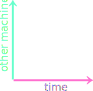
\includegraphics[width=5cm]{Figs/time-vs-machine.pdf}

\end{frame}

\begin{frame}[c]{Tools for R Users}
	In the R Universe and beyond, the most flexible tools are:
  \begin{itemize}
    \item Dynamic document creation = RMarkdown*
    \item Version control = Git**
    \item Workflow management = Make**
    \item Software management = Docker**
  \end{itemize}
  \vfill
  \textcolor{lolit}{
	* RMarkdown supports more then 40 languages e.g.:\\
	\hspace{10mm}Python, Julia, SAS, Scala \& Octave\\
	** Language agnostic
	}
\end{frame}

\begin{frame}[c]{RMarkdown\textemdash{}Literate Programming}
  Text and code are mixed\\
  in a single source document\\
  that can be \textcolor{hilit}{dynamically} compiled\\
  into various representations:
  \begin{itemize}
    \item (APA conformable) manuscripts
    \item presentations
    \item websites
    \item books
    \item posters
		\item CV
  \end{itemize}
\end{frame}

{
  \usebackgroundtemplate{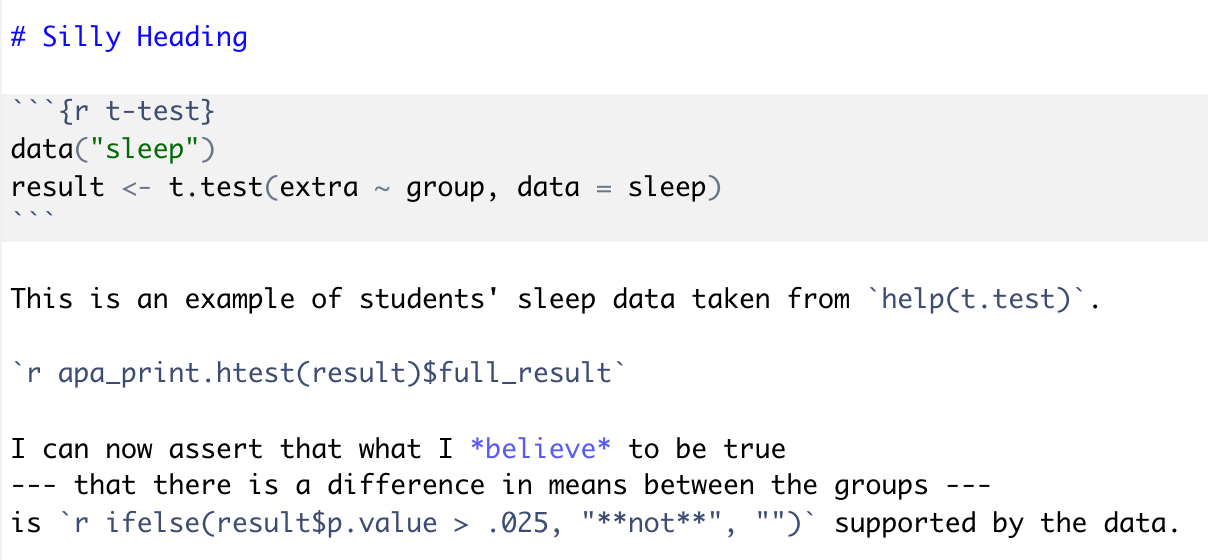
\includegraphics[width=\paperwidth]{Figs/rmarkdown.png}}
  \begin{frame}[plain]
  \end{frame}
}
{
  \usebackgroundtemplate{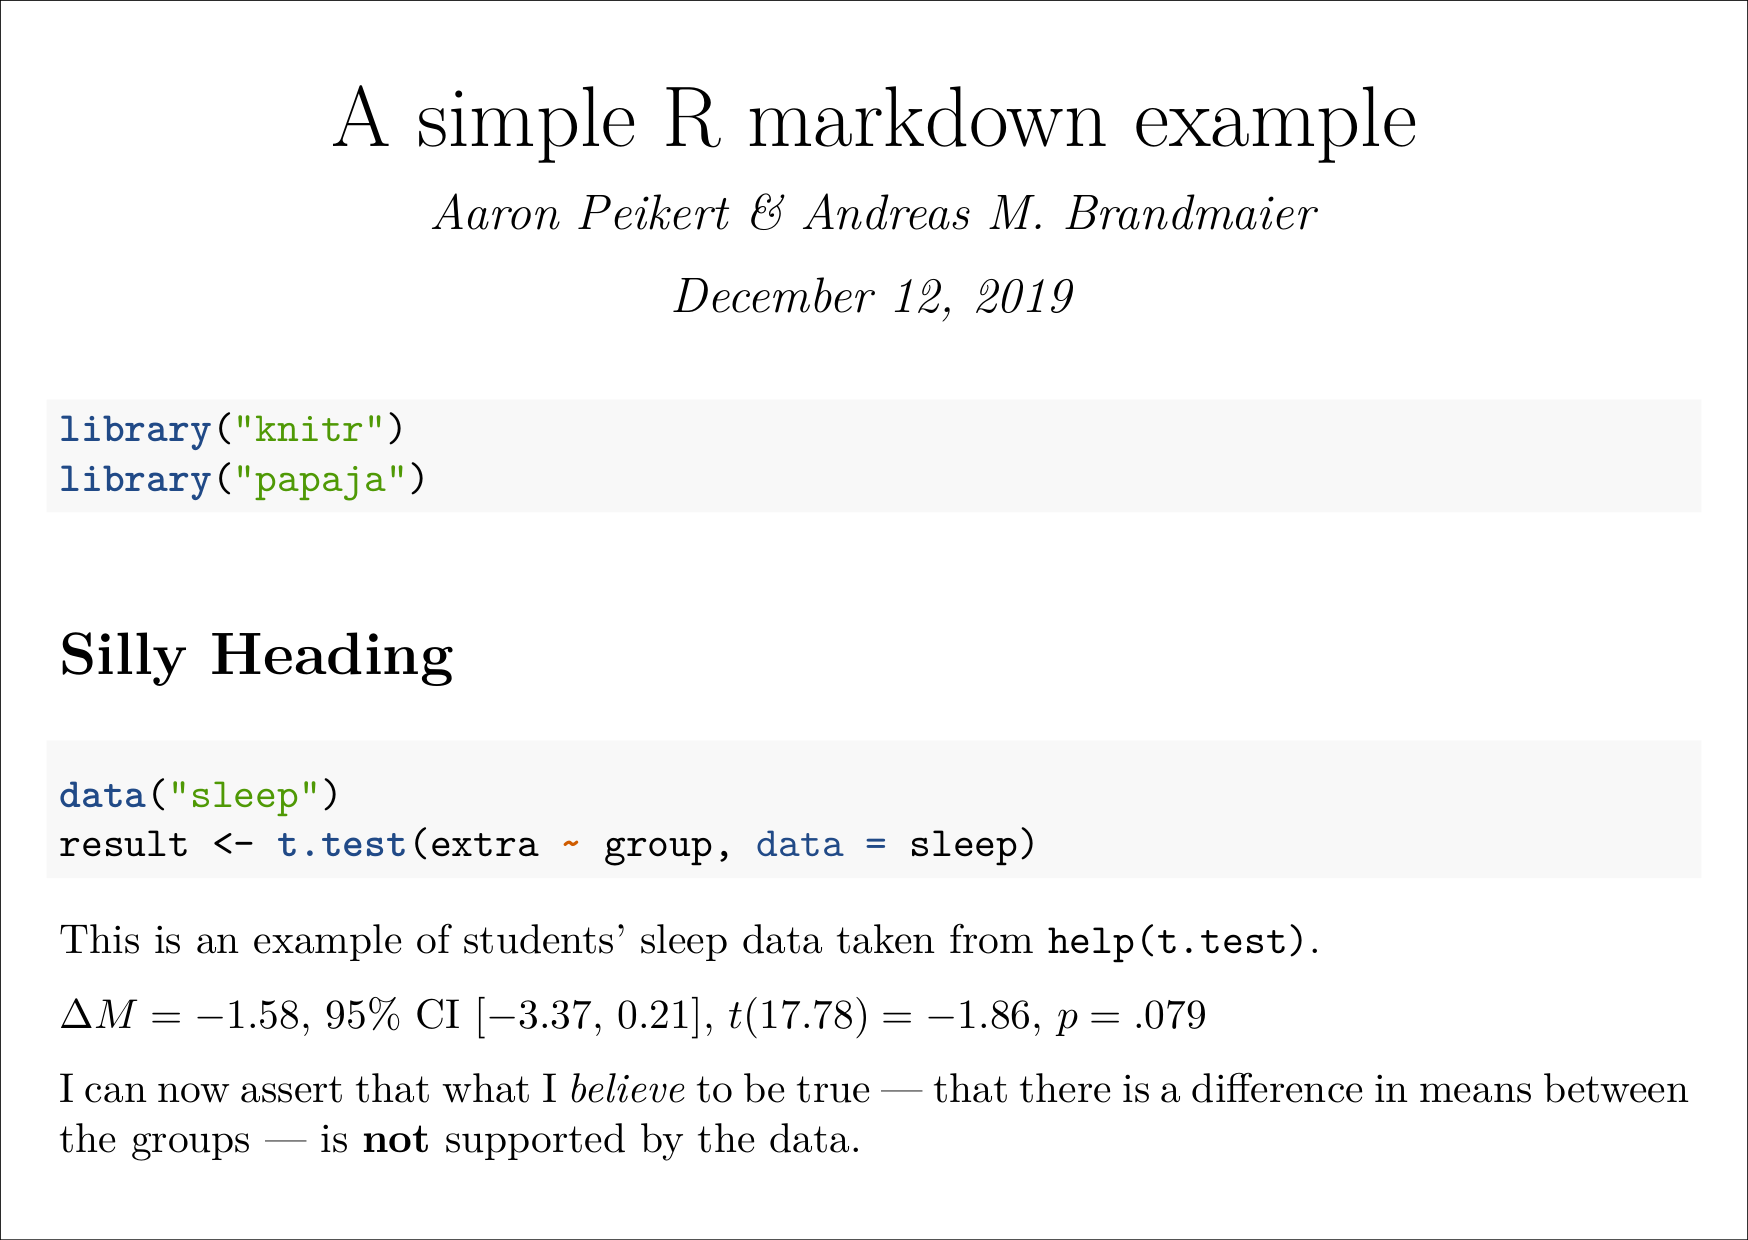
\includegraphics[width=\paperwidth]{Figs/rmarkdown-rendered.png}}
  \begin{frame}[plain]
  \end{frame}
}
\begin{frame}[c]{Git/GitHub\textemdash{}Version Control}
  Version control is a system that records changes to a set of files
  over time so that you can recall specific versions later.\\
  \vspace{10mm}
  It guarantees that code and data are exactly the same version as used for
  publication.
\end{frame}

\begin{frame}[c, fragile]{Make\textemdash{}Workflow management}

Make is a ``recipe" language that describes how files depend on each other and how to resolve these dependencies.
\vspace{10mm}
\begin{lstlisting}[language=make,basicstyle=\ttfamily\scriptsize]
spaghetti_arrabiata.pdf: spagetti_arrabiata.Rmd arrabiata_sauce.csv pasta.csv
    Rscript -e 'rmarkdown::render("spaghetti_arrabiata.Rmd")'

pasta.csv: cook_pasta.R
    Rscript -e 'source("cook_pasta.R")'

arrabiata_sauce.csv: cook_sauce.R canned_tomatoes.csv
    Rscript -e 'source("cook_sauce.R")'
\end{lstlisting}
\end{frame}

\begin{frame}[c, fragile]{Docker\textemdash{}Containerization}
	Docker is a lightweight virtual computer.\\
	Dockerfiles are ``recipes" that describe what to install on that virtual computer:
	\vspace{10mm}
	\begin{lstlisting}[language=make,basicstyle=\ttfamily\scriptsize]
FROM rocker/verse:3.6.1
ARG BUILD_DATE=2019-11-11
RUN install2.r --error --skipinstalled\
  here lavaan
WORKDIR /home/rstudio
\end{lstlisting}
\end{frame}

  \usebackgroundtemplate{\includegraphics[width=\paperwidth]{Figs/nutshell.pdf}}
  \begin{frame}[plain]
  \vspace{8cm}
  \scriptsize \hfill{}\textcolor{black}{From Peikert \& Brandmaier (2019) under CC-BY4.0}
  \end{frame}
}

\begin{frame}[c]{Advantages}
	\begin{center}
		\onslide<1->{\textcolor<2->{lolit}{Unambiguous }}
		\onslide<2->{\textcolor<3->{lolit}{Standardized }}
		\onslide<3->{\textcolor<4->{lolit}{Portable }}
		\onslide<4->{Automated }
	\end{center}
\end{frame}

\begin{frame}[c, fragile]{Simplifying the tools}
\textcolor<2->{lolit}{These tools require extensive training and need much time to configure correctly.\\}
\onslide<2->The R package 'repro' abstracts away the concrete technical implementation:\\
\begin{lstlisting}[basicstyle=\ttfamily\scriptsize]
repro:
  packages:
    - ggplot2
    - aaronpeikert/repro@adb5fa569
  scripts:
    - R/clean.R
  data:
    mycars: data/mtcars.csvrepro:
\end{lstlisting}
The function \lstinline|repro::automate()| automatically infers Docker- and Makefile.
\end{frame}

\begin{frame}[c]{Disadvantages}
\begin{itemize}
	\item requires complex software infrastructure
	\item depends on for-profit services
	\item diverges from the standard manuscript workflow
\end{itemize}
\end{frame}

\begin{frame}[c]{Focus: Computing infrastructure}
	\centering
	\onslide<1>{\textcolor{vhilit}{Workflow management} + \textcolor{hilit}{software management\\}}
	\onslide<1>{=\\}
	\onslide<1->{distributed computation\\}
	\only<2>{\textcolor{vhilit}{\vspace{5mm}Workflow management} enables intelligent task scheduling\\
	\textcolor{hilit}{Software management} guarantees compatible software environment}
	\onslide<3->{on\\}
	\only<3>{Cloud Computing infrastructure\\}
	\only<4>{High Performance Computing cluster (HPC)\\}
\end{frame}

\begin{frame}[c]{HPC\textemdash{}Container}
  \begin{itemize}
  \item repro supports Singularity as a Docker alternative
  \item developing environment matches HPC environment exactly
  \item full freedome to use any software, even when not supported by HPC admin
  \end{itemize}
\end{frame}

\begin{frame}[c]{HPC\textemdash{}Workflow management}
  making dependencies between tasks explicit enables:
  \begin{itemize}
  \item intelligent caching
  \item automatic parralelization
  \item dynamic job scheduling
  \end{itemize}
  \vspace{5mm}
  Make is well supported by several job schedulers.\\
  \vspace{5mm}
  Pure R solutions like the packages \textcolor{vhilit}{targets} + \textcolor{hilit}{futureverse} offer even more convinience and are compatible with repro
\end{frame}

\begin{frame}[c]{Focus: Modularity}
\begin{itemize}
	\item<1-> repro is a modular system
	\item<2-> potential integration of other workflows\\
	\item<3-> ``Lego system of reproducibility tools"
\end{itemize}
\end{frame}

\begin{frame}[c]{Focus: Longterm Archive}
	\textcolor<2>{lolit}{All software is bundled into the container, therefore all we need is:}
	\begin{itemize}
		\item \textcolor<2>{lolit}{container software}
		\item \textcolor<2>{lolit}{storage infrastructure}
	\end{itemize}

	\onslide<2>{
	What happens when Docker and co. are not supported anymore?\\
	Containers can be converted into a full system image ensuring support for decades.
	}

\end{frame}


\begin{frame}[c]{References}
	\textcolor{lolit}{Slides:\\}\href{https://github.com/aaronpeikert/repro-talk}{\texttt{\textcolor{foreground}{https://github.com/aaronpeikert/repro-talk}}}
	\textcolor{lolit}{Package:\\}\href{https://github.com/aaronpeikert/repro-thesis}{\texttt{\textcolor{foreground}{https://github.com/aaronpeikert/repro-thesis}}}\\
	\textcolor{lolit}{Workflow:\\}\href{https://doi.org/10.31234/osf.io/8xzqy}{\texttt{\textcolor{foreground}{https://doi.org/10.31234/osf.io/8xzqy}}}
\end{frame}

\begin{frame}[c]
  \Huge
	\only<1>{Thank you}
	\only<2>{Questions?}
\end{frame}

\end{document}
